\section{Background}
The subsequent section presents background knowledge regarding different concepts and notions that will be adopted throughout the dissertation.
First, a definition of orientation frames and coordinate systems will be presented, followed by an introduction to Euler angles and quaternions, building a foundation of understanding wherein the mathematics and arithmetic behind attitude representation. An introduction to inertial sensors and how they can be employed to estimate orientation is then exhibited. The chapter concludes with an analysis and summary of different sensor fusion algorithms utilized to determine orientation.
\subsection{Frames of coordinates}
This section will focus on defining and distinguishing the different concepts of frame coordinate systems. An emphasis will be given to East North Up (ENU), Earth Centered, Earth Fixed (ECEF) and the World Geodetic System (WGS84). The notion of body frame will also be defined. The ECEF and WGS84 can considered supplementary frame systems applied to describe the ENU frame which can be understood as the world frame.
\subsubsection{ECEF and ENU frame}
ECEF coordinate system describes a referential axis where origin of the coordinates is at the center of mass of the earth, also known as barycenter. Mathematically, this translates to the integral of the position vector times the density over the earth being zero.
\begin{equation}
    \int \overrightarrow{x}\rho~dx^3 = 0
\end{equation}
X-axis is described by the intersection of the zero-latitude line (Equator) plan and the zero-longitude line (prime meridian) plan. The orientation of the X-axis is deemed to be positive from center towards the point defined by zero latitude and zero longitude. Z-axis is expressed by the line interconnecting North and South Poles, staying positive in the direction of the Earth’s barycenter to the North Pole. Y-axis lies in the equatorial plane and is perpendicular to the plan described by X and Z-axis and it is positive direction is defined by right hand rule.
coordinate system is a local coordinate system where the origin is located at a user defined
point in ECEF coordinate system, with Y-axis pointing towards North Pole and X-axis pointing towards
East. The plan defined by X and Y-axis is tangent to the WGS84 frame on the origin of ENU. Z-axis
express the altitude from defined local plane (see figure 2.1). The ENU frame is considered in this work
as the reference frame and will be denoted with superscript or subscript w.
\begin{figure}[!h]
    \centering
    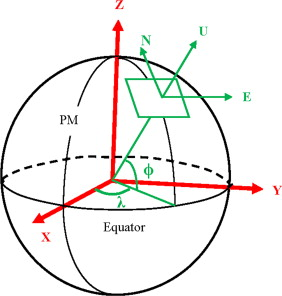
\includegraphics[width=0.7\textwidth]{figures/ECEF.jpg}
    \caption{Representation of the Gimbal Lock problematic \cite{zeitlhofler2019nominal} - The exterior blue gimbal characterizes the x-axis, the middle, red-colored gimbal the y axis, and the inner green gimbal the z-axis. In the initial arrangement a), every axis is perpendicular to one another. Following a rotation of 90º across the red arrow (y-axis), the blue and the green gimbals occupy the same rotation axis. This condition inhibits the clear determination of the rotation axes when subsequently rotating around the x or z-axis. }
    \label{fig:gimballock}
\end{figure}
\subsubsection{Body frame}
Each sensor present in the razor board is aligned to match the sensor axes printed in the board as
seen in figure 3.1. For simplicity, the razor sensors are placed as possible near the middle point of the
bisector segment between the two wheel axes in such a away that YY axis as marked in the figure 3.1
is pointing towards the front of vehicle, XX axis is pointing to the right side of the car and ZZ axis is
pointing to the top. This way, if the Euler angles describing the orientation of body frame related to world
frame are all equal to zero, it means the axes in each frame are coincident apart from an offset in origin.
Rotation angles are considered positive following the right hand rule in each axis. The origin of body
frame is equal to intersection of rear wheel axis with the bisector defined above.
\subsection{Orientation}
The attitude orientation of a UAV is a critical aspect in autonomous flight. In a low-cost
AHRS, accuracy and low complexity are important in calculating the attitude of the UAV.
There are various ways to represent attitude including: Euler angles, quaternions, direct
cosine matrix, and rotational matrix.
\subsubsection{Euler angles}
Euler angles are the easiest to intuitively understand. Euler angles are comprised of three
angles, roll, pitch and yaw. The roll angle $\varphi$  is the axis pointed out the nose and rotates
the plane, along the x-axis. The pitch angle $\varphi$ is the axis pointing out the right wing, and
% represents the inclination and declination of the UAV. Lastly is the yaw angle $\varpsi$ is the axis
pointing out the bottom of the plane, it is used in the calculation of the heading of the UAV.
This representation of Euler angles are shown in figure 2.1.

The order of which the angles are represented in a vector is not important, however the
order of rotation is. The order of rotation used in the implemented Kalman filter algorithm is: roll, pitch, and yaw. The reason for using this ordering is due to how the attitude is
perceived. A UAV in autonomous flight typically does not incline or decline at a high rate,
however it may roll at a high rate. To accurately understand the orientation of the UAV
with respect to the Euler angles, it must be read from the roll first, then pitch, then yaw.
The roll will have the range of ±180◦
, this allows the pitch to have the range of ±90◦
. The
yaw is represented using the range of ±180◦
. The convention is used to keep the accurate
orientation of the plane.

Euler angles have one disadvantage, which is known as Gimbal lock. Euler angles act
as a gimballed system, where the three axes can be thought of as three separate gimbals
connected together. Gimbal lock occurs when two axis are aligned, such as when the plane
is pitched straight up, the pitch an the yaw axis are aligned, and as the roll gimbal is rotated,
the pitch and the yaw angle are both effected the same, therefore losing orientation. The
singularity problem can be fixed by adding another gimbal, or using an ad hoc approach to
hard code values or use limits in the algorithm. The approach used in this thesis is to use a
different representation adding another gimbal, known as quaternions. It is necessary to use
an attitude representation with the least amount of elements because of the low-cost system
requirements of low complexity. Whenever propagating attitude estimation through the
Kalman filter, matrix multiplication increases in comlexity with more elements, especically
in finding the inverse of a matrix.
\subsubsection{Quaternions}
As stated previously, to eliminate the singularities at ±90◦ on the pitch and roll axes, and
to keep the computational efficiency optimal, quaternions are used for state attitude representation. To understand quaternions, one must first understand the complex number
relationship. A complex number can represent a rotation in 2 dimensional coordinate frame
with a real x-axis and imaginary axis y-axis or vise versa.
A quaternion is the same concept, except instead of one imaginary axis, there are three
imaginary axes; in a sense its like combining three complex numbers into one. To go from a
2D interpretation to a 3D, four components are required; one real component qs and three
imaginary qx qy qz which can also be represented as a vector ˜v. Equation (2.1) shows this
relation with the complex number x having a real part a and imaginary part b; and the
quaternion q containing a real scalar part s and an imaginary vector component ~v.
To visualize a quaternion operation, think of Euler angles in the sense that there are
three orthogonal angles each on a separate mutually exclusive axis, x,y and z as shown in
figure 2.2. The rotation is not simultaneous, each rotation must happen sequentially, one
axis at a time. In navigation terms, the plane must roll, then pitch, then yaw. In quaternion
terms, the sequence can be thought of the same way as a rotating a vector laying on the
x-axis, then rotating a vector on the y-axis, and finally rotating a vector on the z-axis.

\subsubsection{Accelerometer}
\subsubsection{Gyroscope}
\subsubsection{Magnetometer}
\subsection{Sensor Fusion}
\subsubsection{Sensor Fusion Algoritms}
\paragraph{Kalman Filter}
The Kalman filter algorithm is a set of mathematical equations that provides a computationally efficient approach to estimate some unknown variables by the detected measurements\cite{welch1995introduction}. Kalman filters operate recursive functions to predict the present state of a linear problem by monitoring the current input data, the previous input data, and the previous state prediction.  Two generally assigned methods for Kalman filter-based sensor fusion are state-vector fusion and measurement fusion. The state-vector fusion method (figure \ref{fig:statekalman}) applies a group of Kalman filters to acquire individual sensor-based state estimates, which are subsequently fused to obtain an enhanced combined state estimate. Measurement fusion (figure \ref{fig:mesearurmentkalman}) approach directly combines the sensor data to achieve a joint measurement and later uses a single Kalman filter to get hold of the final state estimate centered on the fused measurement \cite{mosallaei2007process}.
When applied appropriately, Kalman filters offer highly precise orientation, even with the existence of substantial noise. Nevertheless, Kalman filters are computationally expensive rising hardware cost and latency. They are also of complex implementation, which, shared with computational overhead, can make the algorithm unfeasible for computationally restricted applications. They are regularly useful in a wide-ranging variety of applications and have become a standard method in sensor fusion. Several studies examine the possibility of using Kalman filters to predict a body’s orientation and position by combining multiple sensors. The Kalman filter is founded on recursive Bayesian filtering.
Consequently, the system’s noise is assumed to be Gaussian. Therefore, the Kalman filter is generally suggested for linear systems. For this reason, an extension of the classic Kalman Filter designed for non-linear systems has emerged, recognized as Extended Kalman filter \cite{wilson2019formulation}.


\begin{figure}
    \centering
    \begin{subfigure}[b]{0.45\textwidth}
        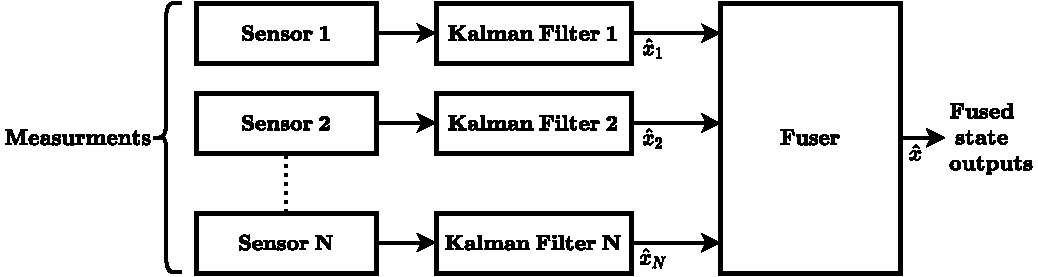
\includegraphics[width=1\linewidth]{figures/kalman1.pdf}
        \caption{}
        \label{fig:statekalman}
    \end{subfigure}
    \begin{subfigure}[b]{0.45\textwidth}
        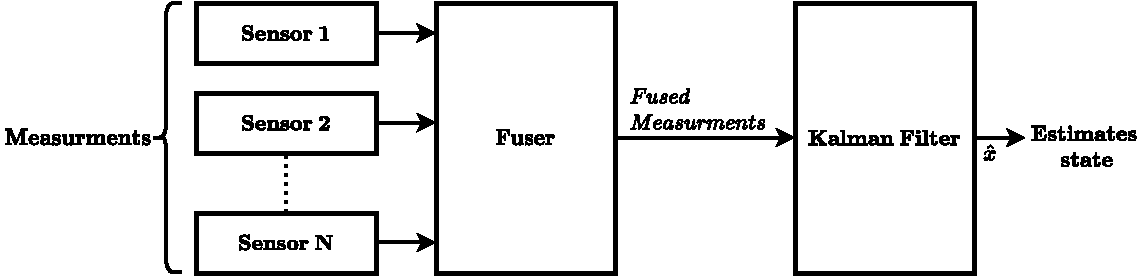
\includegraphics[width=1\linewidth]{figures/kalman2.pdf}
        \caption{}
        \label{fig:mesearurmentkalman}
    \end{subfigure}

    \caption{ Kalman-filter-based multi-sensor data fusion.
        (a) State-vector fusion. (b) Measurement fusion. \cite{mosallaei2007process} }
\end{figure}
\paragraph{Complementary Filter}
The complementary filter is considered a simpler approach relatively to the Kalman filter since it is a computationally lightweight solution and straightforward to implement \cite{higgins1975comparison}. This filter takes as input two noisy sensor measurements and assumes one input is mainly formed by high-frequency signals whereas the other is mostly by low-frequency signals. Through a low pass filter, the high-frequency noise of the first input is filtered out. An identical procedure occurs with the second signal, but this time with a high pass filter to remove low-frequency noises, as illustrated in figure \ref{fig:complementary}. Yet, the complementary filter is not especially robust to noisy or biased data since it simply uses currently available information, therefore, has no direct method of compensating for sensor noise \cite{wilson2019formulation}. A conventional application of the complementary filter is to bring together measurements of vertical acceleration and barometric readings to attain an approximation of vertical velocity. Similar to the Kalman filter, new versions built upon the principles of the classic complementary filter have emerged in recent times, such as the Extended Complementary Filter (ECF). They promise a high level of accuracy and enhanced robustness to noise while preserving computational efficiency.

\begin{figure}[!h]
    \centering
    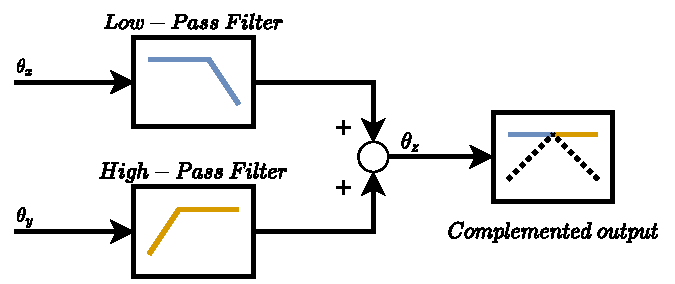
\includegraphics[width=0.7\textwidth]{figures/complementary.pdf}
    \caption{Basic complementary filter \cite{higgins1975comparison} - Two different measurement sources for estimating one variable. The noise properties of the two measurements are such that one source gives good information only in low frequency region while the other is good only in high frequency region. }
    \label{fig:complementary}
\end{figure}

\paragraph{Optimization Filters}
Up until recently, there remained mainly two distinct AHRS fusion approaches. One category including the complementary filters, and the other is related to Kalman filtering. Some recent AHRS algorithms have emerged in the literature over the past years. Two of the most prominent are the Mahony and Madgwick algorithms, which have been categorized as optimization filters. Optimization filters obtain orientation by assessing a vector representative of the sensor output at the present orientation and lessening the disparity concerning predicted and observed outputs. Optimization filters are well established for linking accuracy with computational expense and simplicity of implementation \cite{madgwick2020extended}.
Both methods make use of a quaternion representation, which is a four-dimensional complex number representing of an object orientation. Quaternions involve fewer computation time because of their minimal quantity of calculation parameters \cite{ludwig2018comparison}. Additionally, vector rotations are easily executed by quaternion multiplications.
Madgwick et al. \cite{madgwick2010efficient} pioneered a gradient descent fusion algorithm, frequently recognized as ‘Madgwick Algorithm.’ This gradient descent fusion algorithm first obtains a quaternion estimation of the gyroscope output integration and later corrects it with a quaternion from the accelerometer and magnetometer data. Madgwick’s approach guarantees decent attitude estimation at a low computational cost. Further, it tackles the difficulty of the local magnetic disturbances that can influence all the orientation components. By reducing the constraint of the magnetic field vector rotation, it can limit the effect of the magnetic disturbances to only affect the yaw component of the orientation.

\paragraph{Other Filters}
\subsection{Low-Cost Inertial Measurement Units}
\subsubsection{MPU-9150 Evaluation Board 9DOF}